\documentclass[12pt,
%answers
]{exam}
\usepackage[margin=.8 in]{geometry} 
\usepackage{hyperref,enumerate}
\usepackage{tikz}
\usepackage{amsmath,graphicx, color,comment,amssymb,multicol,cancel}
\newcommand{\tit}{\textit}
\newcommand{\tbf}{\textbf}
\newcommand{\notimplies}{%
  \mathrel{{\ooalign{\hidewidth$\not\phantom{=}$\hidewidth\cr$\implies$}}}}
\newcommand{\ds}{\displaystyle}
\newcommand{\dstyle}{\ds}
\newcommand{\lt}{\left}
\newcommand{\rt}{\right}
\newcommand{\qtq}[1] {\quad \text{#1}\quad}
\newcommand{\Lt}[1]{\mathcal{L} \lt\{ {#1} \rt\}}
\newcommand{\Lti}[1]{\mathcal{L}^{-1} \lt\{ {#1} \rt\}}
\renewcommand{\v}[1]{\vec{\mathbf{#1}}}
\newcommand{\mb}{\mathbf}
\newcommand{\inverse}[1]{ {\mb{#1}}^{-1} }
\makeatletter
\renewcommand*\env@matrix[1][*\c@MaxMatrixCols c]{%
  \hskip -\arraycolsep
  \let\@ifnextchar\new@ifnextchar
  \array{#1}}
\makeatother
\renewcommand{\v}[1]{\vec{\mathbf{#1}}}
\newcommand{\derv}[1]{\vec{\mathbf{#1}}\,' }


\newcounter{quest}


  
% ---- Change the information below ----------------------------------------------------------------------------
\newcommand{\worksheetdate}{ 2024}
%\newcommand{\worksheetdue}{Wednesday, August 24, 2016}
\newcommand{\coursetitle}{}
\newcommand{\worksheettitle}{Graphs of logarithmic functions}
\newcommand{\worksheetsection}{}
% ---- Change the information above ----------------------------------------------------------------------------


%%% adjust space above and below displaymath
\abovedisplayshortskip=0.5em
\belowdisplayshortskip=0.75em
\abovedisplayskip=0.5em
\belowdisplayskip=0.75em
%%% adjust space above and below displaymath


\pagestyle{head}
\runningheadrule \firstpageheader
{\fbox{\parbox{.5\textwidth}{
\textbf{\small Your Name: }
\\ \\ \\ 
%\textbf{Your Name:}
\\
}}}
{}
{\parbox{1.1in}{\fbox{ \parbox{1in}{ \textbf{\small ID \#:  \\  \\ \\ } }}
%\fbox{ \parbox{1in}{ \textbf{\small Section:  \\  } }}
 }}
\runningheader
{{}}%
{\worksheetsection  Page \thepage\ of \numpages}
{\textbf{} \hphantom{\worksheetdate}}

\begin{document}

\newgeometry{top=1.3in, right =0.8in, left=0.8in, bottom =0.8in}

\begin{center}	
{\bf {\coursetitle\,  Worksheet: \worksheettitle} 
	\\ 
	\textbf{}
	\hphantom{\worksheetdate}
%	\worksheetdate
} 		
	\end{center}




\begin{questions}

%%% adjust space above and below displaymath
\abovedisplayshortskip=0.5em
\belowdisplayshortskip=0.75em
\abovedisplayskip=0.5em
\belowdisplayskip=0.75em
%%% adjust space above and below displaymath


\question
Find the  function $f(x)=log_a x$ whose graph is given.
\begin{multicols}{2}
\begin{center}
       \includegraphics[width=4cm]{Images/glpic1.png}
 \end{center}
\columnbreak
\begin{choices}
\choice $f(x)=\log_{\frac{\sqrt{2}}{3}}x$
\choice $f(x)=\log_{\frac{2}{3}}x$
\choice $f(x)=\log_{\frac{3}{2}}x$
\choice $f(x)=\log_{\frac{\sqrt{3}}{2}}x$
\choice none of these
\end{choices}

\end{multicols}

\question
Identify the logarithmic function corresponding to the graph.
\begin{multicols}{2}
\begin{center}
       \includegraphics[width=4cm]{Images/glpic2.png}
 \end{center}
\columnbreak
\begin{choices}
\choice $f(x)=\ln (4+x)$
\choice $f(x)=\ln (x) +4$
\choice $f(x)=\ln(x) -4$
\choice $f(x)=\ln (4-x)$
\choice none of these
\end{choices}

\end{multicols}


\question
Identify the graph of the function $y = \log _3 (x-3)-1$  using the graph of $y=\log_3 x$ shown in then leftmost below.

\includegraphics[width=3.5cm]{Images/glpic3.png}
     \includegraphics[width=3.5cm]{Images/glpic4.png}
          \includegraphics[width=3.5cm]{Images/glpic5.png}
               \includegraphics[width=3.5cm]{Images/glpic6.png}
                    \includegraphics[width=3.5cm]{Images/glpic7.png}
   
  ~\hspace{0.4cm} ($y=\log_3 x$) \hspace{2.2cm} (A)  \hspace{2.8cm} (B) \hspace{3cm} (C) \hspace{3cm} (D)


\question
Determine the graph of the function $f(x)=-4 \ln x$

\includegraphics[width=3.5cm]{Images/glpic8.png}
     \includegraphics[width=3.5cm]{Images/glpic9.png}
          \includegraphics[width=3.5cm]{Images/glpic10.png}
               \includegraphics[width=3.5cm]{Images/glpic11.png}
                    \includegraphics[width=3.5cm]{Images/glpic12.png}
   
  ~\hspace{1cm} (A) \hspace{2.2cm} (B)  \hspace{2.8cm} (C) \hspace{3cm} (D) \hspace{3cm} (E)

\newpage

\question
Match the logarithmic function with one of the graphs labeled I or II.
\begin{multicols}{3}
\begin{center}
\includegraphics[width=4cm]{Images/glpic13.png}
\end{center}
\columnbreak
     \includegraphics[width=4cm]{Images/glpic14.png}
 \columnbreak
 
         I. $f(x)=2+\ln x$ 
         \newline
           II. $f(x)=\ln (x-2)$
\end{multicols}

\question 
Match the functions with graphs

\includegraphics[width=3.5cm]{Images/glpic15.png}
     \includegraphics[width=3.5cm]{Images/glpic16.png}
          \includegraphics[width=3.5cm]{Images/glpic17.png}
               \includegraphics[width=3.5cm]{Images/glpic18.png}
                    \includegraphics[width=3.5cm]{Images/glpic19.png}

\includegraphics[width=3.5cm]{Images/glpic20.png}
     \includegraphics[width=3.5cm]{Images/glpic21.png}
          \includegraphics[width=3.5cm]{Images/glpic22.png} 
          
      \begin{choices}
      \begin{multicols}{4}
          \choice $y=2^x$   
          \choice $y=-\ln x$ \hspace{0.2cm} 
          \columnbreak
       \choice $2x+3y=6$   
        \choice  $y=1-\frac{1}{x^3}$
        \columnbreak
     \choice $y=\log_2 x $    \choice   $y=4e^{-\frac{x^2}{4}}$ 
     \columnbreak
             \choice  $y=2-2x-x^2$     \choice  $y=10xe^{-x}$              
         \end{multicols}
          \end{choices}
\vspace{0.3cm}

\question
Based on the given graph of $f(x)=\log_{\frac{1}{2}}x$, graph $g(x)=f(x)=\log_{\frac{1}{2}}(-x)$ and $h(x)=\log_{\frac{1}{2}}(x-2)+2$

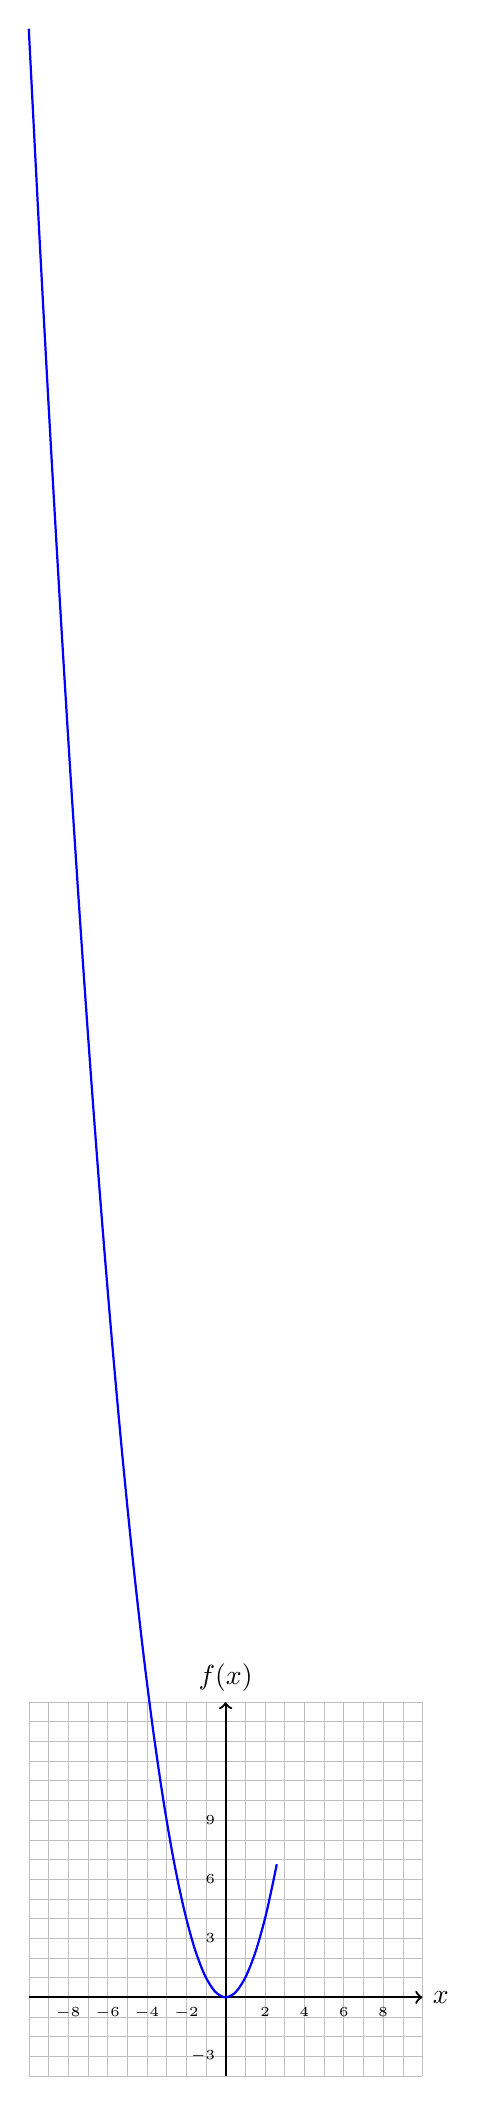
\begin{tikzpicture}[scale=0.25]
\draw[help lines, color=gray!50] (-10,-4) grid (10,15);
\draw[->,thick] (-10,0)--(10,0) node[right]{$x$};
\draw[->, thick] (0,-4)--(0,15) node[above]{$f(x)$};
\foreach \x in {-8,-6,-4,-2,2,4,6,8}
\draw (\x cm,0.25pt) -- (\x cm,-0.25 pt) node[anchor=north] {\tiny{$\x$}};
\foreach \y in {-3,3,6,9}
\draw (1pt,\y cm) -- (-1pt,\y cm) node[anchor=east] {\tiny{$\y$}};
\draw[scale=1, domain=-10:2.6, smooth, variable=\x, thick, blue] plot ({\x},{(\x)^2});
\end{tikzpicture}


\end{questions}
\end{document}






